\section{Applications and Evaluation}
\label{sec:eval}

We have implemented the interpolation algorithm in a modified version of the \dReal which is currently available at \url{https://github.com/dzufferey/dreal3/}\footnote{Once the implementation is stable, the interpolation will be merged into the released, main repository of \dReal}.
Since the proofs produced by \dReal can be very large,i.e., gigabytes, the interpolants are built and simplified on-the-fly.
We modified the ICP loop and the contractors which are responsible for the pruning steps.
The full proof is not kept.

\paragraph{Flyspeck benchmarks.}
\todo{change the name of that paragraph}
The ICP algorithm eagerly contract the domain by applying repeatedly \emph{all} the constraints. Therefore, it usually generate large proofs often involving all the constraints and all the variables.
Interpolation can extract more precise information from the proof.
Intuitively, an interpolant which is much smaller than the proof are more likely to be useful in practice.
In this test, we try to compare the size of the proof against the size of the interpolants using benchmark from the Flyspeck project~\cite{???} and the other examples presented in the rest of this Section.

The Flyspeck project~\cite{???} as build a mechanized proof of the Kepler conjecture.
Part of the proof requires showing the unsatisfiability of nonlinear formulas.
In previous work~\cite{???}, part of these formulas were translated to the input format of \dReal.
We use this example as they provide a large number of tests and allow us to get quantitative information about our interpolation algorithm.

We run \dReal, with a 10 minute timeout, and generate XXX interpolants.
Out of these, XXX are nontrivial.
\todo{update those two numbers once we are done}
In Figure~\ref{fig:flyspeck} we plot the number of inequalities in the nontrivial interpolants against the size of the proof.
For similar proofs, we see that the interpolants can be order of magnitude simpler than the proofs and other interpolants obtained by different partitions of the formula.
The trivial interpolants still bring information as they means that the only one side is part of the unsatisfiable core.


\begin{figure}
\centering
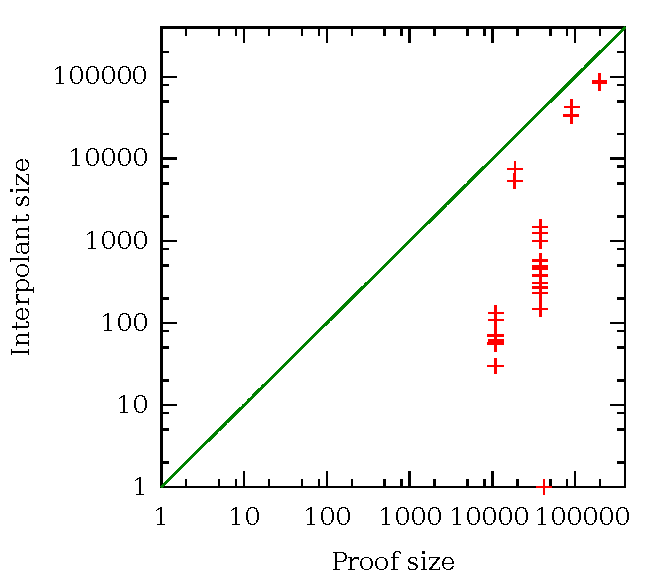
\includegraphics[scale=0.6]{img/itpsize2.pdf}
\caption{
    Size of the interpolants (number of inequalities) compared to the size of the proof.
}
\label{fig:flyspeck}
\end{figure}


\paragraph{Hybrid system verification.}
... ToDo: rather about ODE than hybrid part ...

Figure~\ref{fig:ode} shows an interpolant obtained for the following system of ODEs:
\begin{eqnarray*}
A: &~~~~&  x_t = x₀ + \int_0^t \! -x + cos(x) \, \mathrm{d}x ∧ x₀ = 3 ∧ 0 ≤ t ≤ 2 \\
B: &~~~~&  y_t = y₀ + \int_0^t \! -y + sin(y-1) \, \mathrm{d}y ∧ y₀ = 2 ∧ x_t = y_t
\end{eqnarray*}

\begin{figure}
\centering
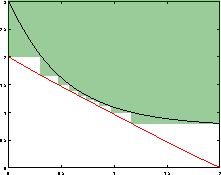
\includegraphics[scale=1.5]{img/ode.pdf}
\caption{ Interpolant for system of nonlinear ODEs }
\label{fig:ode}
\end{figure}

\todo[inline]{a table for other ode examples}

\paragraph{Robotic design.}
Most of the time, hybrid system verification is built around model-based design.
An expert produces a model of the system which is then verified.
However, it is also possible to extract models directly from the manufacturing designs.
As part of an ongoing project about co-design of both the software and hardware parts of robots~\cite{react}, we extract equations from robotic designs.
In the extracted model, each structural element is represented by a 3D vector for position and a unit quaternion for the orientation.
The dimension of the elements and the joints connecting them corresponds to equations that appropriately relate the position and orientation variables.
Active elements, such as motors, also have specific equations associated to them.

This approach has own sets of challenges as we get large system of very details equations.
To verify such systems, we need to simplify them.
Due to the presence of trigonometric functions we cannot use quantifier elimination for polynomial systems of equations~\cite{qepcad}.
However, we can use interpolation as an approximation of quantifier elimination.

Let us consider a kinematic model, $𝓚(\vec x,\vec y,\vec z)$ where $\vec x$ is a set of design and input parameters, $\vec y$ is the variables that represent the state of each component of the robot, and $\vec z$ is the variables that represent the part of the state needed to prove the property of interest.

For instance, in the case of a robotic manipulator, $\vec x$ contain the size of the element and the angles of the servo motors and $\vec z$ is the position of the effector.
$\vec y$ is determined by the designed of the manipulator.

The model we use satisfy the property that once the design and input parameters are fixed, there is a unique solution for the model.
Therefore, we can create an interpolation query:
\begin{eqnarray*}
A: &~~~~ &  𝓚(\vec x,\vec y,\vec z) ∧ \\
B: &~~~~ &  𝓚(\vec x,\vec v,\vec w) ∧ (\vec z-\vec w)² ≥ ε² \quad \text{where} ~ ε > δ
\end{eqnarray*}
$\vec y, \vec v$ are two copies of the variables we want to eliminate.
Since the kinematic is a function of $\vec x$ which is the same for the two copies $\vec z$ and $\vec w$ should be equal.
Therefore, the formula we build has no solution and we get an interpolant $I(\vec x,\vec z)$ which is an ε-approximation of $∃ \vec y.\,𝓚(\vec x,\vec y,\vec z)$.

\begin{example}
Consider the simple robotic manipulator show in Figure~\ref{fig:robot}.
The manipulator is composed of two beams connected by a revolute joint controlled by a servo motor.
The first beam is fixed.

The original system of equations describing this system has 22 variables: 7 for each beam, 7 for the effector, and 1 for the revolute joint.
Using the interpolation we obtain a simpler formula with only 4 variables: 3 for the effector's position and 1 for the joint.
Table~\ref{tbl:robot} shows some statistics about the interpolants we obtained using different ε for a one and a two degrees of freedom manipulators.


\begin{figure}
\centering
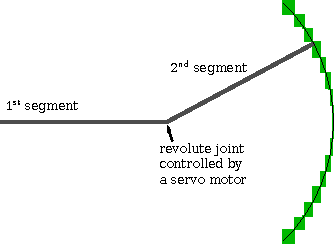
\includegraphics[scale=1]{img/arm.pdf}
\caption{
    Model of a simple robotic manipulator with one degree of freedom composed of 2 segments.
    The segments are 100mm long.
    The black line shows the effector's reach and the green cubes are the approximation obtained by interpolation where ε is 10mm.
}
\label{fig:robot}
\end{figure}

\begin{table}
\centering
\begin{tabular}{l|clrr}
1-DOF Model & ~ \#var  ~~ & Theory   & \#th.~atoms & ~~ time \\
\hline
\hline
original & 22 & polynomial deg.~2, trig.~fct.   & 24    & - \\
\hline
ε = 10   & 4  & linear                          & 1073  & 0.3s \\
ε = 5    & 4  & linear                          & 2757  & 0.6s \\
ε = 3    & 4  & linear                          & 3307  & 0.8s \\
ε = 2    & 4  & linear                          & 6137  & 1.3s \\
ε = 1    & 4  & linear                          & 12485 & 2.6s \\
\end{tabular}

\vspace{2ex}

\begin{tabular}{l|clrr}
2-DOF Model    & ~ \#var  ~~ & Theory   & \#th.~atoms & ~~ time \\
\hline
\hline
original & 30 & polynomial deg.~2, trig.~fct.   & 32        & - \\
\hline
ε = 10   & 5  & linear                          & 45686     & 2m\,7s \\
ε = 7    & 5  & linear                          & 97068     & 3m\,51s  \\
ε = 5    & 5  & linear                          & 184762    & 6m\,41s  \\
ε = 3    & 5  & linear                          & 547558    & 19m\,4s  \\
ε = 2    & 5  & linear                          & 1151454   & 41m\,51s  \\
\end{tabular}

\vspace{1ex}

\caption{
    Comparison of the original model of a 1 and 2 degrees of freedom manipulator against approximations obtained using interpolation.
    For the size of the formulas we report the number of theory atoms in the formula.
    The last column shows the time \dReal takes to compute the interpolants.
}
\label{tbl:robot}
\end{table}


\end{example}





